\documentclass[tikz,border=12pt]{standalone}
\usepackage[T1]{fontenc}
\usepackage{helvet}
\renewcommand{\familydefault}{\sfdefault}
\usepackage{amsmath}
\usetikzlibrary{arrows.meta, fit, backgrounds, positioning, calc, shapes.geometric}

% Semantic palette: teal = dense / neural step (embedding, cosine search,
% reranker); gray = neutral glue / query; amber = stores; green = output.
\definecolor{queryfill}{HTML}{ECEFF2}
\definecolor{queryborder}{HTML}{8A96A3}
\definecolor{encfill}{HTML}{DCEFE9}
\definecolor{encborder}{HTML}{2E9478}
\definecolor{corpusfill}{HTML}{FBF0D5}
\definecolor{corpusborder}{HTML}{CFA23E}
\definecolor{outfill}{HTML}{E7F4E7}
\definecolor{outborder}{HTML}{59A05B}
\definecolor{poolfill}{HTML}{F1F9F1}
\definecolor{regfill}{HTML}{F6F8FB}
\definecolor{regborder}{HTML}{C4CDD6}
\definecolor{darkline}{HTML}{333333}
\definecolor{subtext}{HTML}{5A5A5A}

\tikzset{
  card/.style={rectangle, rounded corners=5pt, align=center, draw=darkline,
               line width=0.8pt, minimum height=1.2cm, font=\small},
  query/.style={card, fill=queryfill, draw=queryborder, minimum width=2.0cm},
  enc/.style={card, fill=encfill, draw=encborder, minimum width=2.5cm},
  result/.style={card, fill=outfill, draw=outborder, minimum width=2.2cm},
  leaf/.style={rectangle, rounded corners=3pt, draw=outborder, fill=outfill,
               line width=0.8pt, minimum width=1.05cm, minimum height=0.78cm, font=\scriptsize},
  db/.style={cylinder, shape border rotate=90, aspect=0.28, draw=corpusborder,
             fill=corpusfill, line width=0.8pt, minimum width=1.75cm,
             minimum height=1.05cm, font=\scriptsize, align=center, inner sep=1pt},
  region/.style={rounded corners=12pt, fill=regfill, draw=regborder, line width=0.8pt},
  pooldash/.style={draw=outborder, dashed, rounded corners=8pt, fill=poolfill,
                   line width=0.85pt},
  regtitle/.style={font=\small\bfseries, text=darkline},
  note/.style={font=\scriptsize\itshape, text=subtext, align=center},
  flow/.style={-{Latex[length=2.2mm]}, line width=0.85pt, draw=darkline},
  feed/.style={-{Latex[length=1.9mm]}, line width=0.7pt, draw=corpusborder},
}

\def\pspread{0.88cm}

\begin{document}
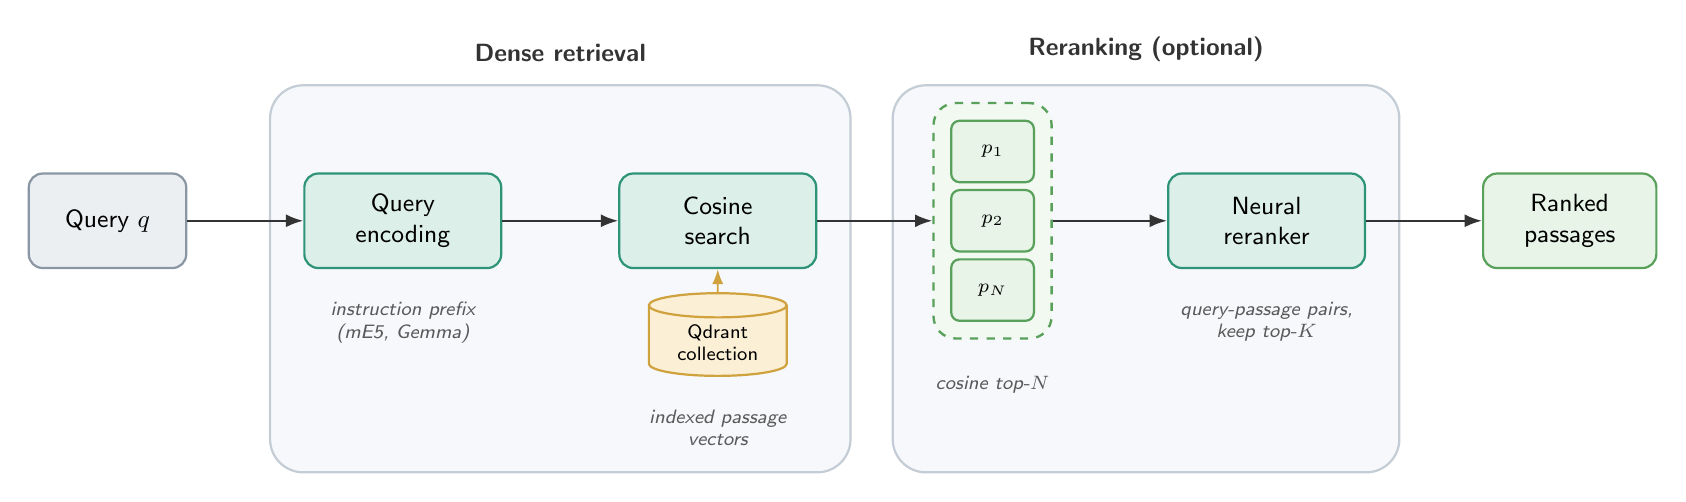
\begin{tikzpicture}

% Spine: query, encode, search, pool, rerank, output all on y=0. The x-positions
% give a uniform 1.5cm edge-to-edge gap between every box, so all the connector
% arrows are the same length. The inter-panel separation comes from panel padding.
\node[query] (query)  at (0,0)    {Query $q$};
\node[enc]   (qenc)   at (3.75,0) {Query\\encoding};
\node[enc]   (cosine) at (7.75,0) {Cosine\\search};
\node[db]    (qdrant) at (7.75,-1.55) {Qdrant\\collection};

% Candidate pool: cosine top-N, fed to the reranker
\node[leaf] (p1) at (11.24, \pspread)  {$p_1$};
\node[leaf] (p2) at (11.24, 0)         {$p_2$};
\node[leaf] (pn) at (11.24,-\pspread)  {$p_N$};
\node[font=\footnotesize] at ($(p2)!0.5!(pn)$) {$\vdots$};
\node[pooldash, fit=(p1)(p2)(pn), inner sep=6pt] (pool) {};
\foreach \n/\t in {p1/p_1, p2/p_2, pn/p_N} { \node[leaf] at (\n) {$\t$}; }

\node[enc]    (rerank)  at (14.72,0) {Neural\\reranker};
\node[result] (sources) at (18.57,0) {Ranked\\passages};

% Notes
\node[note, below=0.30cm of qenc]   (qencnote)   {instruction prefix\\(mE5, Gemma)};
\node[note, below=0.30cm of qdrant] (qdrantnote) {indexed passage\\vectors};
\node[note, below=0.34cm of pool]   (poolnote)   {cosine top-$N$};
\node[note, below=0.30cm of rerank] (reranknote) {query-passage pairs,\\keep top-$K$};

% Phase panels, made equal in height. Dense retrieval extends up to the pool
% top, reranking extends down to the Qdrant-note bottom, so both rectangles span
% the same vertical band. Input and output stay outside.
\begin{scope}[on background layer]
  \coordinate (bandT) at (pool.north);
  \coordinate (bandB) at (qdrantnote.south);
  \node[region, inner xsep=12pt, inner ysep=6pt,
        fit=(qenc)(qencnote)(cosine)(qdrant)(qdrantnote)(qenc|-bandT)] (reg1) {};
  \node[region, inner xsep=12pt, inner ysep=6pt,
        fit=(pool)(poolnote)(rerank)(reranknote)(rerank|-bandB)] (reg2) {};
\end{scope}
\node[regtitle, anchor=south] at ($(reg1.north)+(0,0.16)$) {Dense retrieval};
\node[regtitle, anchor=south] at ($(reg2.north)+(0,0.16)$) {Reranking (optional)};

% Flow
\draw[flow] (query) -- (qenc);
\draw[flow] (qenc.east) -- (cosine.west);
\draw[feed] (qdrant.north) -- (cosine.south);
\draw[flow] (cosine.east) -- (pool.west);
\draw[flow] (pool.east) -- (rerank.west);
\draw[flow] (rerank.east) -- (sources.west);

\end{tikzpicture}
\end{document}
